\documentclass[oneside,12pt,fancychapters]{scrbook} %%%%mine
\usepackage[utf8]{inputenc}
\usepackage{minitoc} %to get mini table of contents for each chapter
\usepackage{hyperref} %hyperlinks

\usepackage{graphicx}
\usepackage{subcaption}
\usepackage{subfigure}


\title{Roombee Manual}
\author{Marcus Futterlieb}
\date{20.01.2016}

\pdfinfo{%
  /Title    (roombee manual)
  /Author   (Marcus Futterlieb)
  /Creator  (Marcus Futterlieb) 
  /Producer (Marcus Futterlieb)
  /Subject  (mobile robotics)
  /Keywords (mobile robotics, drive by odometry, diy robot)
}

\begin{document}
\dominitoc
\maketitle

\tableofcontents

\chapter{Disclaimer}
This software has been developed to allow curious owners of a iRobot Roomba 500 series to gather some experience in the domain of mobile robotics. 
A serious help in the development was "The MATLAB Toolbox for the iRobot Create" which can be found \href{http://www.usna.edu/Users/weapsys/esposito/roomba-matlab.php}{here}.
The author can not be held responsible for any damage caused directly or indirectly by the software. 


\chapter{Prerequisites and Requirements}
In order to use this software you need a few things.
Apart from the robot (you can find cheap offers of used robots on ebay, or your local equivalent) and a laptop you will need:
\begin{itemize}
  \item A working Matlab version (all above 2012b should work fine)
  \item A serial connection (USB to serial is sufficient, however you can find offers that provide a serial to blue-tooth connection)
  \item (optional) Some kind of small platform you can mount on the robot to provide a more reliable base for your laptop
\end{itemize}

\chapter{Get the Robot operational}
Here I want to explain how to get your iRobot Roomba modified in order to use the code properly.
First of all you will have to remove the cover lid in order to gain access to the serial plug.
This is necessary to control the robot with your laptop.
Figures~\ref{fig:general1} and~\ref{fig:general2} show the Roomba without the lid and with an added plexiglass table to accommodate my laptop. 
Following this a view of the operational Roombee platform is given (Figures~\ref{fig:laptop_mounted1} and~\ref{fig:laptop_mounted2}).
The final images in Figure~\ref{fig:setup_1} show the serial to USB cable.



\begin{figure}
\centering     %%% not \center
\subfigure[Modified Roomba, cover lid removed]{\label{fig:general1}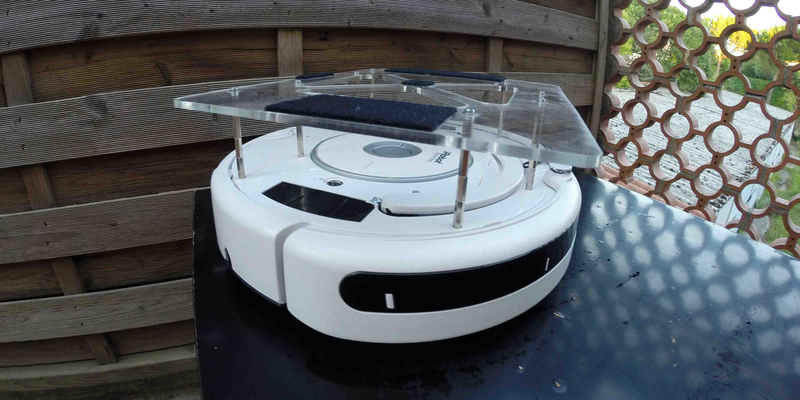
\includegraphics[width=0.45\textwidth]{media/resized/0.png}}
\subfigure[Modified Roomba, cover lid removed]{\label{fig:general2}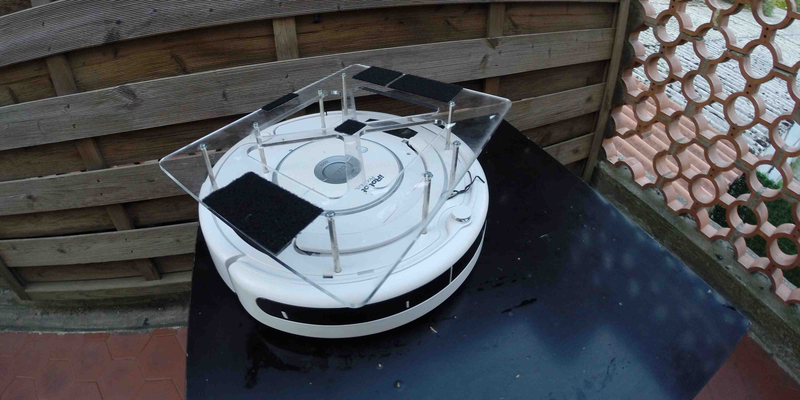
\includegraphics[width=0.45\textwidth]{media/resized/6.png}}
\subfigure[Laptop mounted on plexiglass table]{\label{fig:laptop_mounted1}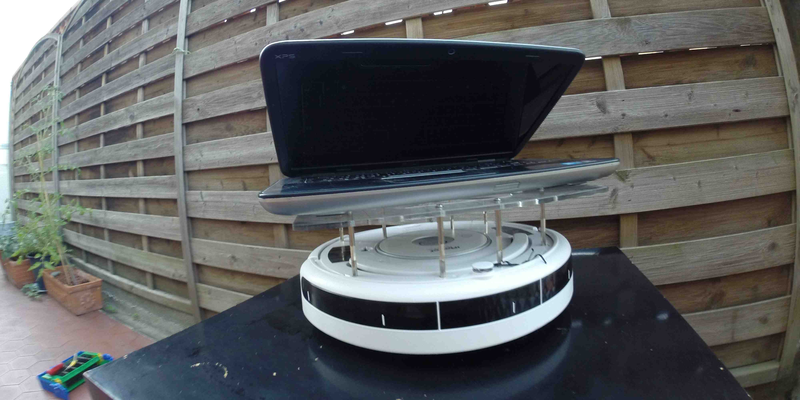
\includegraphics[width=0.45\textwidth]{media/resized/7.png}}
\subfigure[Laptop mounted on plexiglass table]{\label{fig:laptop_mounted2}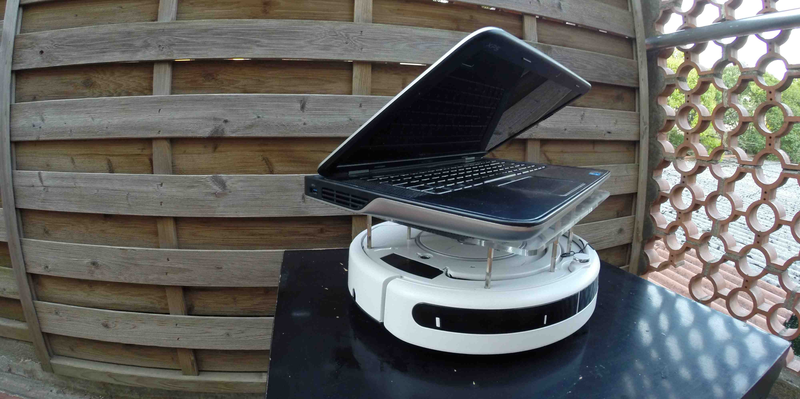
\includegraphics[width=0.45\textwidth]{media/resized/8.png}}
\subfigure[Roomba and serial to USB cable]{\label{fig:cable1}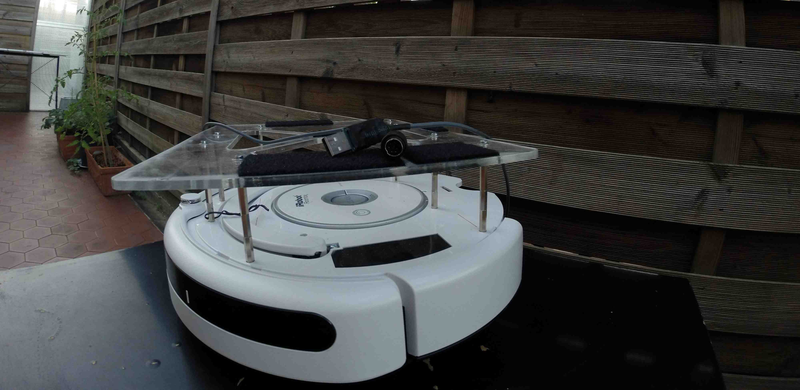
\includegraphics[width=0.45\textwidth]{media/resized/4.png}}
\subfigure[Roomba and serial to USB cable]{\label{fig:cable2}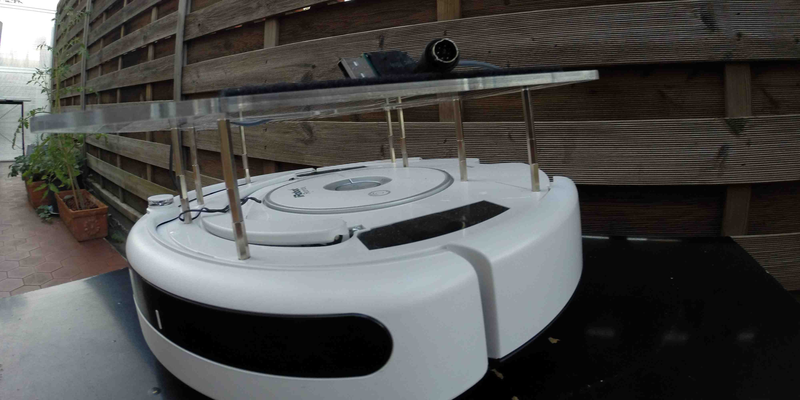
\includegraphics[width=0.45\textwidth]{media/resized/3.png}}
\caption{General overview of the platform}
\label{fig:setup_1}
\end{figure}



\begin{figure}
\centering     %%% not \center
\subfigure[Turn your Roomba upside down]{\label{fig:upside_down1}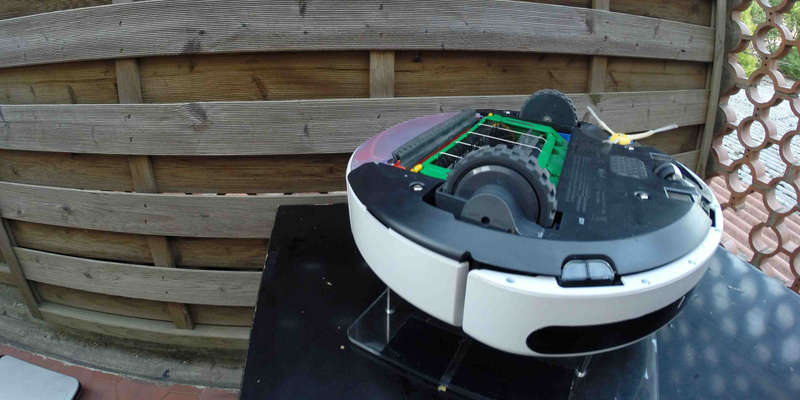
\includegraphics[width=0.45\textwidth]{media/resized/10.png}}
\subfigure[Locate the corner brush]{\label{fig:upside_down2}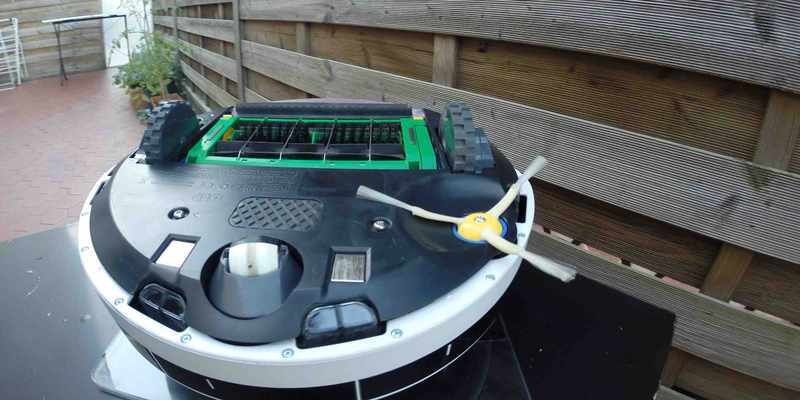
\includegraphics[width=0.45\textwidth]{media/resized/9.png}}
\subfigure[Remove screw to remove corner brush]{\label{fig:remove_corner_brush}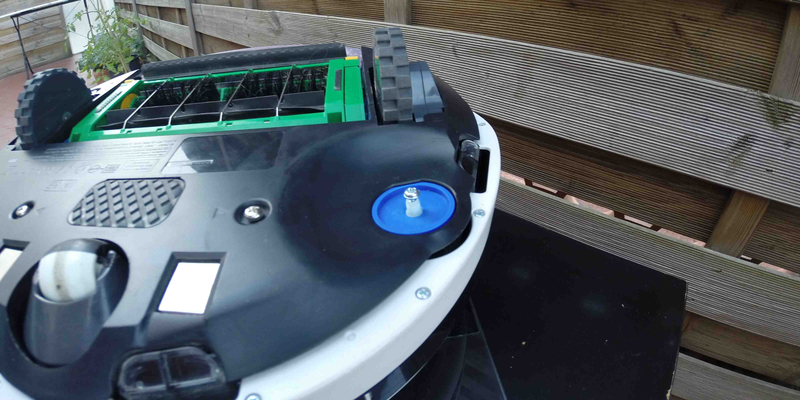
\includegraphics[width=0.45\textwidth]{media/resized/11.png}}
\subfigure[Remove the dust container]{\label{fig:remove_dust_container}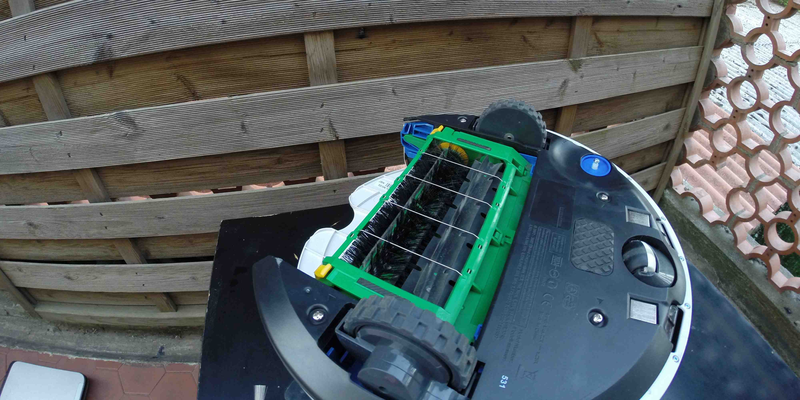
\includegraphics[width=0.45\textwidth]{media/resized/12.png}}
\subfigure[Remove the underbody cover lid to gain access to the battery and main brushes]{\label{fig:remove underbody}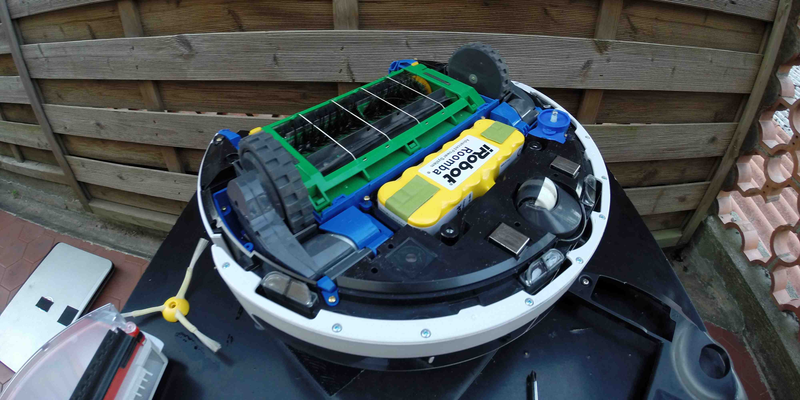
\includegraphics[width=0.45\textwidth]{media/resized/13.png}}
\subfigure[Take out the main brush system]{\label{fig:b}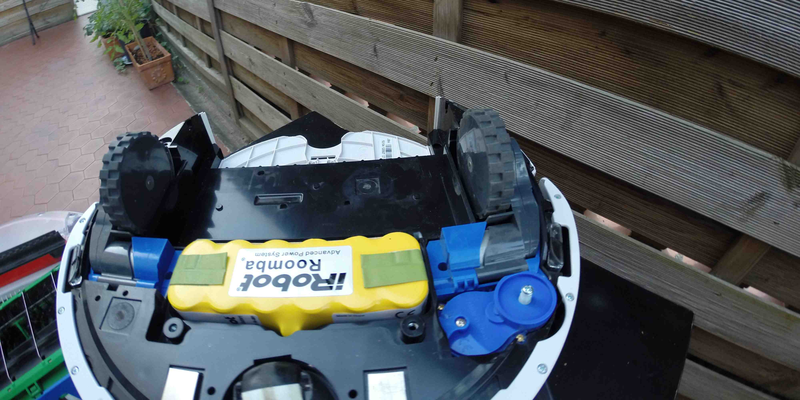
\includegraphics[width=0.45\textwidth]{media/resized/14.png}}

\subfigure[Re-attach the underbody lid and the dust container]{\label{fig:b}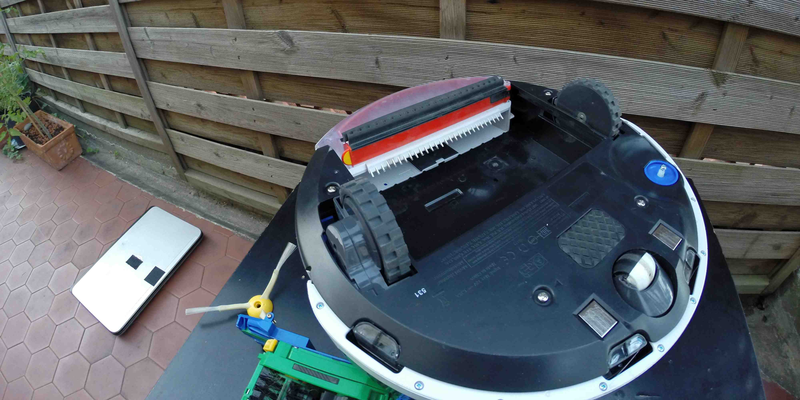
\includegraphics[width=0.45\textwidth]{media/resized/1.png}}
\subfigure[Your robot is now operational]{\label{fig:upside_down}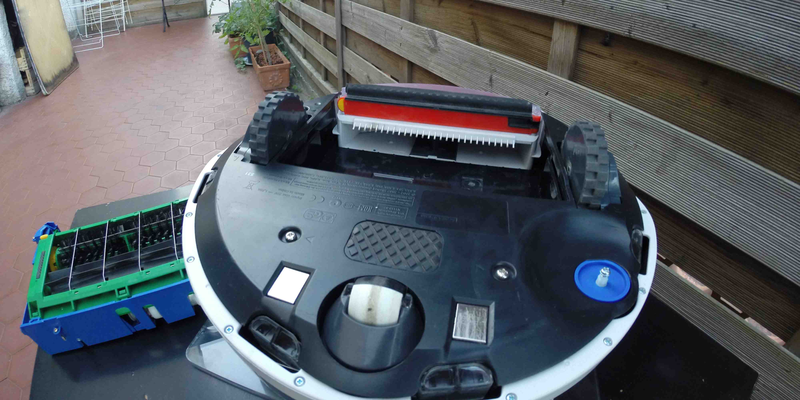
\includegraphics[width=0.45\textwidth]{media/resized/2.png}}

\caption{Remove Roomba cleaning equipment to gain battery autonomy}
\label{fig:setup_2}
\end{figure}


\chapter{How to use the Code}
\chapter{How to create the Light Graffiti Effect}
The tool used for post processing the video material is \href{https://kdenlive.org/}{Kdenlive}.
It should be accessible through the apt-get command.
Once installed it handles much like any other video editing software.
The effect you are looking for is called "Light Graffiti" and can be found under:\\
\textbf{Effect List/Misc/ Light Graffiti} \\
You have to choose your parameters so that the brightest point in the video is the light source in the center of the robot.
A head lamp for camping should be sufficient. 


\vspace {0.5cm}

Examples can be found at:

\begin{itemize}
  \item \href{https://youtu.be/hPpPM0kasyk}{Youtube video of a Roomba following a certain letter sequence indoors}
  \item \href{https://youtu.be/g-6yrYu4PUs}{Youtube video of a Roomba following a certain letter sequence outdoors}
\end{itemize}


\chapter{Outlook}
In the future several modifications are planned. 
First of all a remote will be build that allows to control the robot with an xbox controller, but switch to execute a task autonomously whenever 
necessary. 

\end{document}
